% Options for packages loaded elsewhere
\PassOptionsToPackage{unicode}{hyperref}
\PassOptionsToPackage{hyphens}{url}
%
\documentclass[
]{article}
\usepackage{amsmath,amssymb}
\usepackage{iftex}
\ifPDFTeX
  \usepackage[T1]{fontenc}
  \usepackage[utf8]{inputenc}
  \usepackage{textcomp} % provide euro and other symbols
\else % if luatex or xetex
  \usepackage{unicode-math} % this also loads fontspec
  \defaultfontfeatures{Scale=MatchLowercase}
  \defaultfontfeatures[\rmfamily]{Ligatures=TeX,Scale=1}
\fi
\usepackage{lmodern}
\ifPDFTeX\else
  % xetex/luatex font selection
\fi
% Use upquote if available, for straight quotes in verbatim environments
\IfFileExists{upquote.sty}{\usepackage{upquote}}{}
\IfFileExists{microtype.sty}{% use microtype if available
  \usepackage[]{microtype}
  \UseMicrotypeSet[protrusion]{basicmath} % disable protrusion for tt fonts
}{}
\makeatletter
\@ifundefined{KOMAClassName}{% if non-KOMA class
  \IfFileExists{parskip.sty}{%
    \usepackage{parskip}
  }{% else
    \setlength{\parindent}{0pt}
    \setlength{\parskip}{6pt plus 2pt minus 1pt}}
}{% if KOMA class
  \KOMAoptions{parskip=half}}
\makeatother
\usepackage{xcolor}
\usepackage[left=30mm,right=30mm]{geometry}
\usepackage{longtable,booktabs,array}
\usepackage{calc} % for calculating minipage widths
% Correct order of tables after \paragraph or \subparagraph
\usepackage{etoolbox}
\makeatletter
\patchcmd\longtable{\par}{\if@noskipsec\mbox{}\fi\par}{}{}
\makeatother
% Allow footnotes in longtable head/foot
\IfFileExists{footnotehyper.sty}{\usepackage{footnotehyper}}{\usepackage{footnote}}
\makesavenoteenv{longtable}
\usepackage{graphicx}
\makeatletter
\def\maxwidth{\ifdim\Gin@nat@width>\linewidth\linewidth\else\Gin@nat@width\fi}
\def\maxheight{\ifdim\Gin@nat@height>\textheight\textheight\else\Gin@nat@height\fi}
\makeatother
% Scale images if necessary, so that they will not overflow the page
% margins by default, and it is still possible to overwrite the defaults
% using explicit options in \includegraphics[width, height, ...]{}
\setkeys{Gin}{width=\maxwidth,height=\maxheight,keepaspectratio}
% Set default figure placement to htbp
\makeatletter
\def\fps@figure{htbp}
\makeatother
\setlength{\emergencystretch}{3em} % prevent overfull lines
\providecommand{\tightlist}{%
  \setlength{\itemsep}{0pt}\setlength{\parskip}{0pt}}
\setcounter{secnumdepth}{-\maxdimen} % remove section numbering
\ifLuaTeX
  \usepackage{selnolig}  % disable illegal ligatures
\fi
\IfFileExists{bookmark.sty}{\usepackage{bookmark}}{\usepackage{hyperref}}
\IfFileExists{xurl.sty}{\usepackage{xurl}}{} % add URL line breaks if available
\urlstyle{same}
\hypersetup{
  hidelinks,
  pdfcreator={LaTeX via pandoc}}

\author{}
\date{}

\begin{document}

\section{Computational Methods}\label{computational-methods}

\subsection{Task 1 - Brute Force}\label{task-1---brute-force}

\begin{figure}
\centering
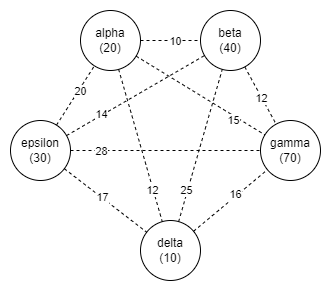
\includegraphics[width=0.5\textwidth,height=\textheight]{diagrams/bruteforce_diagram.png}
\caption{Diagram of the planets as a graph}
\end{figure}

A program was written to brute-force this, as opposed to doing it by
hand. Below is the pseudocode.

\begin{verbatim}
Let adjacency_matrix = {{0,10,15,12,20}, 
                        {10,0,12,25,14}, 
                        {15,12,0,16,28}, 
                        {12,25,16,0,17}, 
                        {20,14,28,17,0}}
Let cargo_pickup_weights = [20,40,70,10,30]

Function get_distance(a, b):
    Return adjacency_matrix[a][b]
End Function

Function calculate_fuel_cost(a, b, c, d, e):
    Let total_fuel = 0
    Let total_weight = 0

    total_weight = total_weight + cargo_pickup_weights[a]
    total_fuel = total_fuel + get_distance(a,b)*total_weight

    total_weight = total_weight + cargo_pickup_weights[b]
    total_fuel = total_fuel + get_distance(b,c)*total_weight

    total_weight = total_weight + cargo_pickup_weights[c]
    total_fuel = total_fuel + get_distance(c,d)*total_weight

    total_weight = total_weight + cargo_pickup_weights[d]
    total_fuel = total_fuel + get_distance(d,e)*total_weight

    total_weight = total_weight + cargo_pickup_weights[e]

    Return total_fuel*25
End Function

Let all_possible_sequences = []

Let a = 0
While a < 5:
    Let sequence = [a]

    Let b = 0
    While b < 5:
        If sequence Contains b:
            Continue
        End If
        Append b to sequence

        Let c = 0
        While c < 5:
            If sequence Contains c:
                Continue
            End If
            Append c to sequence

            Let d = 0
            While d < 5:
                If sequence Contains d:
                    Continue
                End If
                Append d to sequence

                Let e = 0
                While e < 5:
                    If sequence Contains e:
                        Continue
                    End If
                    Append e to sequence

                    Append sequence to all_possible_sequences
                    sequence = [a,b,c,d]
                    Increment e
                End While
                sequence = [a,b,c]
                Increment d
            End While
            sequence = [a,b]
            Increment c
        End While
        sequence = [a]
        Increment b
    End While

    Increment a
End While

Open "brute_force.csv" as file
Let index = 0
While index < Length of all_possible_sequences:
    Let seq = all_possible_sequences[index]
    Output seq[0] to file
    Output "," to file
    Output seq[1] to file
    Output "," to file
    Output seq[2] to file
    Output "," to file
    Output seq[3] to file
    Output "," to file
    Output seq[4] to file
    Output "," to file
    Output calculate_fuel_cost(seq[0], seq[1], seq[2], seq[3], seq[4]) to file
    Output "\n" to file
End While

Close file
\end{verbatim}

Below is the equivalent python code.

\begin{verbatim}
alpha = 0
beta = 1
gamma = 2
delta = 3
epsilon = 4

adjacency_matrix = [[0,10,15,12,20], 
                    [10,0,12,25,14], 
                    [15,12,0,16,28], 
                    [12,25,16,0,17], 
                    [20,14,28,17,0]]

cargo_pickup_weights = [20,40,70,10,30]

def get_distance(a, b):
    return adjacency_matrix[a][b]

def calculate_fuel_cost(a, b, c, d, e):
    total_fuel = 0
    total_weight = 0
    
    total_weight += cargo_pickup_weights[a]
    total_fuel += get_distance(a,b)*total_weight

    total_weight += cargo_pickup_weights[b]
    total_fuel += get_distance(b,c)*total_weight

    total_weight += cargo_pickup_weights[c]
    total_fuel += get_distance(c,d)*total_weight

    total_weight += cargo_pickup_weights[d]
    total_fuel += get_distance(d,e)*total_weight

    total_weight += cargo_pickup_weights[e]

    return total_fuel*25


all_possible_sequences = []

for a in range(5):
    sequence = [a]
    for b in range(5):
        if (b in sequence): continue
        sequence.append(b)
        for c in range(5):
            if (c in sequence): continue
            sequence.append(c)
            for d in range(5):
                if (d in sequence): continue
                sequence.append(d)
                for e in range(5):
                    if (e in sequence): continue
                    sequence.append(e)
                    all_possible_sequences.append(sequence)
                    sequence = [sequence[0], sequence[1], sequence[2], sequence[3]]
                sequence = [sequence[0], sequence[1], sequence[2]]
            sequence = [sequence[0], sequence[1]]
        sequence = [sequence[0]]
                    
csv_data = ""
for seq in all_possible_sequences:
    csv_data += str(seq[0]) + ","
    csv_data += str(seq[1]) + ","
    csv_data += str(seq[2]) + ","
    csv_data += str(seq[3]) + ","
    csv_data += str(seq[4]) + ","
    csv_data += str(calculate_fuel_cost(seq[0], seql[1], seq[2], seq[3], seq[4])) + "\n"

print("generated " + str(len(all_possible_sequences)) + " sequences")

file = open("brute_force.csv", "w")

file.write(csv_data)
file.close()
\end{verbatim}

See the CSV file which is produced by the python program, and a more
formatted Excel conversion.

\url{c025180n_brute_force.csv}

\url{c025180n_brute_force.xlsx}

Reading from the generated files, it can be seen that the cheapest route
is
\texttt{3\ 0\ 4\ 1\ 2\ =\ Delta\ -\textgreater{}\ Alpha\ -\textgreater{}\ Epsilon\ -\textgreater{}\ Beta\ -\textgreater{}\ Gamma},
which costs 69000 intergalactic currency.

This approach isn't a good way to find the shortest path since it
requires checking the cost of an enormous and rapidly increasing search
space. Specifically \(n!\) possible routes, \(n\) being the number of
planets (Flood, 1956)\footnote{Flood, M. M. (1956), \emph{`The
  Traveling-Salesman Problem.',} \emph{Operations Research}, 4(1),
  pp.~61--75. Available at: http://www.jstor.org/stable/167517
  (Accessed: 20 November 2023).}; this is because there are \(n\)
possible planets for the first destination, \(n-1\) for the second, etc.
Factorial time, \(O(n!)\) is a bad time complexity. In order to evaluate
the cost of each route, the program also has to traverse the whole list
of planets representing each route, which are length \(n\), so the real
time complexity is \(O(n\times n!)\). Optimisations which can be applied
are limited since the problem is analogous to the asymmetric travelling
salesman problem (i.e.~reversed routes are not equal in cost), however
we could reduce the number of routes to be checked using a dynamic
programming approach, by exploring the graph gradually and comparing
partial routes with the same planets visited and the same end planet.
This could reduce the time complexity to \(O(n^2 2^{n-1})\), but with
much worse space complexity (Bellman, 1962)\footnote{Bellman, R. (1962)
  \emph{`Dynamic programming treatment of the travelling salesman
  problem'}, \emph{Journal of the ACM}, 9(1), pp.~61--63.
  doi:10.1145/321105.321111.}.

\newpage

\subsection{Task 2 - Sorting}\label{task-2---sorting}

\begin{longtable}[]{@{}
  >{\raggedright\arraybackslash}p{(\columnwidth - 30\tabcolsep) * \real{0.0256}}
  >{\raggedright\arraybackslash}p{(\columnwidth - 30\tabcolsep) * \real{0.0256}}
  >{\raggedright\arraybackslash}p{(\columnwidth - 30\tabcolsep) * \real{0.0256}}
  >{\raggedright\arraybackslash}p{(\columnwidth - 30\tabcolsep) * \real{0.0256}}
  >{\raggedright\arraybackslash}p{(\columnwidth - 30\tabcolsep) * \real{0.0256}}
  >{\raggedright\arraybackslash}p{(\columnwidth - 30\tabcolsep) * \real{0.0256}}
  >{\raggedright\arraybackslash}p{(\columnwidth - 30\tabcolsep) * \real{0.0256}}
  >{\raggedright\arraybackslash}p{(\columnwidth - 30\tabcolsep) * \real{0.0256}}
  >{\raggedright\arraybackslash}p{(\columnwidth - 30\tabcolsep) * \real{0.0256}}
  >{\raggedright\arraybackslash}p{(\columnwidth - 30\tabcolsep) * \real{0.0256}}
  >{\raggedright\arraybackslash}p{(\columnwidth - 30\tabcolsep) * \real{0.0427}}
  >{\raggedright\arraybackslash}p{(\columnwidth - 30\tabcolsep) * \real{0.0256}}
  >{\raggedright\arraybackslash}p{(\columnwidth - 30\tabcolsep) * \real{0.0256}}
  >{\raggedright\arraybackslash}p{(\columnwidth - 30\tabcolsep) * \real{0.0256}}
  >{\raggedright\arraybackslash}p{(\columnwidth - 30\tabcolsep) * \real{0.0940}}
  >{\raggedright\arraybackslash}p{(\columnwidth - 30\tabcolsep) * \real{0.5299}}@{}}
\toprule\noalign{}
\begin{minipage}[b]{\linewidth}\raggedright
0
\end{minipage} & \begin{minipage}[b]{\linewidth}\raggedright
1
\end{minipage} & \begin{minipage}[b]{\linewidth}\raggedright
2
\end{minipage} & \begin{minipage}[b]{\linewidth}\raggedright
3
\end{minipage} & \begin{minipage}[b]{\linewidth}\raggedright
4
\end{minipage} & \begin{minipage}[b]{\linewidth}\raggedright
5
\end{minipage} & \begin{minipage}[b]{\linewidth}\raggedright
6
\end{minipage} & \begin{minipage}[b]{\linewidth}\raggedright
7
\end{minipage} & \begin{minipage}[b]{\linewidth}\raggedright
8
\end{minipage} & \begin{minipage}[b]{\linewidth}\raggedright
9
\end{minipage} & \begin{minipage}[b]{\linewidth}\raggedright
start
\end{minipage} & \begin{minipage}[b]{\linewidth}\raggedright
end
\end{minipage} & \begin{minipage}[b]{\linewidth}\raggedright
i
\end{minipage} & \begin{minipage}[b]{\linewidth}\raggedright
j
\end{minipage} & \begin{minipage}[b]{\linewidth}\raggedright
pivot value
\end{minipage} & \begin{minipage}[b]{\linewidth}\raggedright
notes
\end{minipage} \\
\midrule\noalign{}
\endhead
\bottomrule\noalign{}
\endlastfoot
10 & 15 & 12 & 12 & 25 & 16 & 20 & 14 & 28 & 17 & 0 & 9 & -1 & 10 & 25 &
partition the whole list \\
& & & & & & & & & & & & 0 & 10 & & \\
& & & & & & & & & & & & 1 & 10 & & \\
& & & & & & & & & & & & 2 & 10 & & \\
& & & & & & & & & & & & 3 & 10 & & \\
& & & & & & & & & & & & 4 & 10 & & \\
& & & & & & & & & & & & 4 & 9 & & \\
10 & 15 & 12 & 12 & 17 & 16 & 20 & 14 & 28 & 25 & & & & & & swap 4 and
9 \\
& & & & & & & & & & & & 5 & 9 & & \\
& & & & & & & & & & & & 6 & 9 & & \\
& & & & & & & & & & & & 7 & 9 & & \\
& & & & & & & & & & & & 8 & 9 & & \\
& & & & & & & & & & & & 8 & 8 & & \\
& & & & & & & & & & & & 8 & 7 & & partitioning finished \\
10 & 15 & 12 & 12 & 17 & 16 & 20 & 14 & & & 0 & 7 & -1 & 8 & 12 &
subsort first half \\
& & & & & & & & & & & & 0 & 8 & & \\
& & & & & & & & & & & & 1 & 8 & & \\
& & & & & & & & & & & & 1 & 7 & & \\
& & & & & & & & & & & & 1 & 6 & & \\
& & & & & & & & & & & & 1 & 5 & & \\
& & & & & & & & & & & & 1 & 4 & & \\
& & & & & & & & & & & & 1 & 3 & & \\
10 & 12 & 12 & 15 & 17 & 16 & 20 & 14 & & & & & & & & swap 1 and 3 \\
& & & & & & & & & & & & 2 & 3 & & \\
& & & & & & & & & & & & 2 & 2 & & \\
& & & & & & & & & & & & 2 & 1 & & partitioning finished \\
10 & 12 & & & & & & & & & 0 & 1 & -1 & 2 & 10 & subsort first half of
first half \\
& & & & & & & & & & & & 0 & 2 & & \\
& & & & & & & & & & & & 0 & 1 & & \\
& & & & & & & & & & & & 0 & 0 & & subsort done \\
& & 12 & 15 & 17 & 16 & 20 & 14 & & & 2 & 7 & 1 & 8 & 17 & subsort
second half of first half \\
& & & & & & & & & & & & 2 & 8 & & \\
& & & & & & & & & & & & 3 & 8 & & \\
& & & & & & & & & & & & 4 & 8 & & \\
& & & & & & & & & & & & 4 & 7 & & \\
& & 12 & 15 & 14 & 16 & 20 & 17 & & & & & & & & swap 4 and 7 \\
& & & & & & & & & & & & 5 & 7 & & \\
& & & & & & & & & & & & 6 & 7 & & \\
& & & & & & & & & & & & 6 & 6 & & \\
& & & & & & & & & & & & 6 & 5 & & partitioning finished \\
& & 12 & 15 & 14 & 16 & & & & & 2 & 5 & 1 & 6 & 15 & subsort first half
of second half of first half \\
& & & & & & & & & & & & 2 & 6 & & \\
& & & & & & & & & & & & 3 & 6 & & \\
& & & & & & & & & & & & 3 & 5 & & \\
& & & & & & & & & & & & 3 & 4 & & \\
& & 12 & 14 & 15 & 16 & & & & & & & & & & swap 3 and 4 \\
& & & & & & & & & & & & 4 & 4 & & \\
& & & & & & & & & & & & 4 & 3 & & partitioning finished \\
& & 12 & 14 & & & & & & & 2 & 3 & 1 & 4 & 12 & subsort first half of
first half of second half of first half \\
& & & & & & & & & & & & 2 & 4 & & \\
& & & & & & & & & & & & 2 & 3 & & \\
& & & & & & & & & & & & 2 & 2 & & subsort done \\
& & & & 15 & 16 & & & & & 4 & 5 & 3 & 6 & 15 & subsort second half of
first half of second half of first half \\
& & & & & & & & & & & & 4 & 6 & & \\
& & & & & & & & & & & & 4 & 5 & & \\
& & & & & & & & & & & & 4 & 4 & & subsort done \\
& & & & & & 20 & 17 & & & 6 & 7 & 5 & 8 & 20 & subsort second half of
second half of first half \\
& & & & & & & & & & & & 6 & 8 & & \\
& & & & & & & & & & & & 6 & 7 & & \\
& & & & & & 17 & 20 & & & & & & & & swap 6 and 7 \\
& & & & & & & & & & & & 7 & 7 & & \\
& & & & & & & & & & & & 7 & 6 & & subsort done \\
& & & & & & & & 28 & 25 & 8 & 9 & 7 & 10 & 28 & subsort second half \\
& & & & & & & & & & & & 8 & 10 & & \\
& & & & & & & & & & & & 8 & 9 & & \\
& & & & & & & & & & & & & & & swap 8 and 9 \\
& & & & & & & & 25 & 28 & & & & & & \\
& & & & & & & & & & & & 9 & 9 & & \\
& & & & & & & & & & & & 9 & 8 & & subsort done \\
10 & 12 & 12 & 14 & 15 & 16 & 17 & 20 & 25 & 28 & & & & & & sort done \\
\end{longtable}

This trace table represents a quicksort, and below is the pseudocode for
it.

\begin{verbatim}
Procedure swap(array, first, second) Begin:
    Let temp = array[first]
    array[first] = array[second]
    array[second] = temp
End Procedure

Function partition_array(array, start, end) Begin:
    // Place the pivot in the middle, this tends to have better performance
    Let pivot_index = ((end - start)/2 Rounded Down) + start
    Let pivot = array[pivot_index]
    
    // Initialise pointers
    Let i = start - 1
    Let j = end + 1
    
    While True:
        // Increment i then break if the targeted element is swappable
        While True:
            Increment i
            If array[i] >= pivot:
                Break
            End If
        End While
        
        // Decrement j then break if the targeted element is swappable
        While True:
            Decrement j
            If array[j] <= pivot:
                Break
            End If
        End While
        
        // Return the partition point if i and j meet/cross, otherwise swap their values
        If i >= j:
            Return j
        Else:
            swap(array, i, j)
        End If
    End While
End Function

Procedure quick_sort(array, start, end) Begin:
    // Return if there is nothing to sort
    If start >= end:
        Return
    End If
    
    // Perform first sorting pass over current whole array
    Let split_index = partition_array(array, start, end)
    
    // Perform subsorts on partitioned arrays
    quick_sort(array, start, split_index)
    quick_sort(array, split_index + 1, end)
End Procedure
\end{verbatim}

This is an implementation of the quicksort algorithm, using Hoare's
pivot choice and pair-of-pointers method (Hoare, 1962)\footnote{Hoare,
  C. A. R. (1962) \emph{`Quicksort'},~\emph{The Computer Journal}, 5(1),
  pp.~10--16. doi:10.1093/comjnl/5.1.10.}. It makes use of recursive
quicksort calls to sort a list by swapping items so that they
effectively end up grouped (in each sublist) in groups of larger and
smaller items; these sublists can then be sorted using the same method,
until there is only one item in each sublist (this is the trivial base
case for the recursion), as described by Hoare, the designer of the
algorithm. This is an example of a divide-and-conquer approach, as the
subsequent quicksorts can be parallelised, since they are independent
from one another (Esau Taiwo et al., 2020)\footnote{Esau Taiwo, O.
  \emph{et al.} (2020) \emph{`Comparative study of two divide and
  conquer sorting algorithms: Quicksort and Mergesort'}, \emph{Procedia
  Computer Science}, 171, pp.~2532--2540.
  doi:10.1016/j.procs.2020.04.274.}. Quicksort, depending on
implementation (particularly choice of pivot) as well as how sorted data
already is, usually has worst-case complexity \(O(n^2)\). Quicksort also
has the advantage that the pointer loops inside
\texttt{partition\_array} can be implemented very efficiently on current
standard computer architecture (Deshmukh \& Bhavsar, 2020)\footnote{Deshmukh,
  S.M., Bhavsar, A.K. (2020) \emph{`A Review on Different Quicksort
  Algorithms'}, \emph{International Journal of Science, Spirituality,
  Business and Technology}, 7(2), pp.~3--7.}. With Hoare's partitioning
scheme using the middle-pivot (as opposed to pivoting at the start or
end value) tends to have average-case complexity of \(O(n \log_2(n))\),
often better, and rare worst-case complexity of \(O(n^2)\); the
worst-case can be further avoided by pivoting on the median of the
first, middle, and last elements in the list (Fouz et al.,
2011)\footnote{Fouz, M. \emph{et al.} (2011) \emph{`On smoothed analysis
  of~quicksort~and~Hoare's find'}, \emph{Algorithmica}, 62(3--4),
  pp.~879--905. doi:10.1007/s00453-011-9490-9.}.

\newpage

\subsection{Task 3 - Greedy Strategy}\label{task-3---greedy-strategy}

\begin{figure}
\centering
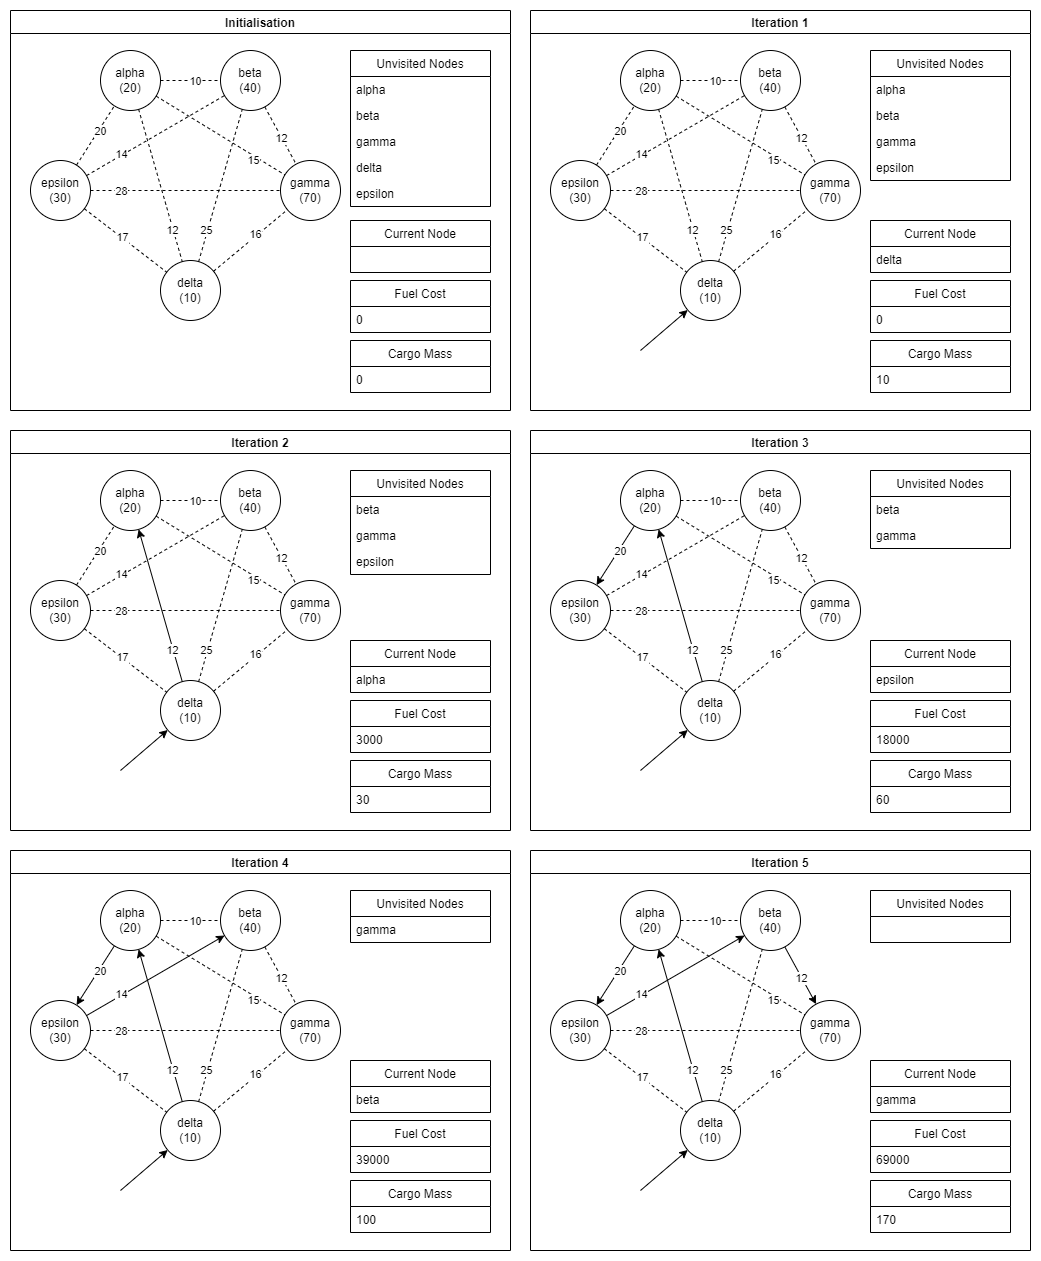
\includegraphics[width=0.75\textwidth,height=\textheight]{diagrams/greedy_diagram_new.png}
\caption{Process of traversing the graph using a mass-focused greedy
strategy}
\end{figure}

\newpage

A greedy strategy chooses the best option in the short term without
looking ahead, so two approaches were considered: first, traversing the
graph by moving along the \textbf{shortest distance edge} to an adjacent
unvisited node; second, to traverse along the edge to the \textbf{lowest
cargo mass} (using mass here to be distinct from edge weights)
\textbf{adjacent unvisited} node. Each of these methods would repeat
until all nodes have been visited. This produces an \(O(n(n-1))\)
traversal in both cases, traversing \(n\) nodes and checking \(n-1\)
other nodes at each step to decide where to traverse next, which is much
better than the \(O(n!)\) offered by brute-force. These strategies
represent a variation of the nearest neighbour algorithm, NND, as this
task is analogous to TSP (Kizilateş \& Nuriyeva, 2013)\footnote{Kizilateş,
  G., Nuriyeva, F. (2013) \emph{`On the nearest neighbor algorithms for
  the traveling salesman problem'}, \emph{Advances in Intelligent
  Systems and Computing}, pp.~111--118.
  doi:10.1007/978-3-319-00951-3\_11.}. The second method produced the
route (starting at delta, since it has the lowest cargo mass)
\texttt{delta\ -\textgreater{}\ alpha\ -\textgreater{}\ epsilon\ -\textgreater{}\ beta\ -\textgreater{}\ gamma},
costing \textbf{69000}, which is coincidentally the optimal path found
by brute-force. The first approach, starting at the same place, resulted
in
\texttt{delta\ -\textgreater{}\ gamma\ -\textgreater{}\ beta\ -\textgreater{}\ alpha\ -\textgreater{}\ epsilon},
which costs almost double the other method at \textbf{126500}
intergalactic currency. It follows common sense that a mass-focused
route would be better, since mass accumulates during the journey,
whereas the edge weightings (distances between planets) do not
accumulate. Although a greedy strategy is not guaranteed to find the
optimal solution (Vince, 2002)\footnote{Vince, A. (2002) \emph{`A
  framework for the greedy algorithm'}, \emph{Discrete Applied
  Mathematics}, 121(1--3), pp.~247--260.
  doi:10.1016/s0166-218x(01)00362-6.}, it will find a reasonably good
solution (a local minimum) in polynomial time (Abdulkarim \& Alshammari,
2015)\footnote{Abdulkarim, H.A., Alshammari, I.F., (2015)
  \emph{`Comparison of algorithms for solving traveling salesman
  problem.'}~\emph{International Journal of Engineering and Advanced
  Technology},~4(6), pp.~76-79.}. The problem is considerably simplified
by the fact that no consideration is needed for the cargo or fuel
capacity for the spaceship, as other similar problems (like F-GVRP) must
consider refueling (Poonthalir \& Nadarajan, 2018)\footnote{Poonthalir,
  G., Nadarajan, R. (2018) \emph{`A fuel efficient green vehicle routing
  problem with varying speed constraint (F-GVRP)'}, \emph{Expert Systems
  with Applications}, 100, pp.~131--144. doi:10.1016/j.eswa.2018.01.052.}.

In the implementation, planets are stored as \textbf{structures},
containing all the information about them and how they connect,
eliminating the need for many list lookups. It was found that,
surprisingly, when constructing the list of connections that each node
has with other nodes, it's \emph{better} to not sort the list by cargo
mass (which would reduce searching later). The later loop not only needs
to find the next lowest cargo mass planet, it needs to \emph{find one
which is unvisited}, meaning it performs a linear search through the
connected planets regardless. This means choosing between either an
\(O(n^3)\) sorting pass with an \(O(n^2)\) traversal pass, or an
\(O(n^2)\) preparation pass with an \(O(n^2)\) traversal pass, the
latter of which is better. Thus the resulting algorithmic complexity of
this solution is \(O(n^2)\), due to the two occurrences of traversing
lists of length \(n\), \(n\) times over. The pseudocode and C++
implementation are below.

\begin{verbatim}
Let NUM_PLANETS = 5
Let FUEL_COST = 25

// structure holding data about a planet (i.e. a node)
Structure planet
    Let name = ""
    Let index = 0
    Let cargo_mass = 0
    Let links = {}
End Structure

// starting data about the planets
Let node_names = { "alpha", "beta", "gamma", "delta", "epsilon" }
Let cargo_masses = { 20,40,70,10,30 }
Let adjacency_matrix = { {0,10,15,12,20}, 
                         {10,0,12,25,14}, 
                         {15,12,0,16,28}, 
                         {12,25,16,0,17}, 
                         {20,14,28,17,0} }

// initialise the nodes in the graph
Let planets = {}
Let i = 0
While i < NUM_PLANETS
    Let p = Create planet
    name Of p = node_names[i]
    cargo_mass Of p = cargo_masses[i]
    index Of p = i
    Append p To planets
    
    Increment i
End While

Let p_minimum = planets[0]

// setup links between nodes
For p_origin In planets

    // update the lowest cargo mass planet
    // since we want to start at this planet
    // and this saves using a second loop
    If cargo_mass Of p_origin < cargo_mass Of p_minimum
        p_minimum = p_origin
    End If

    // add links from this node to all other nodes
    // but not itself
    Let i = 0
    While i < NUM_PLANETS
        If planets[i] Not p_origin
            Let distance = adjacency_matrix[i][index Of p_origin]
            Append {planets[i], distance} To links Of p_origin
        End If
        Increment i
    End While
End For

// traverse the graph, keeping track of which planets
// have been visited, and which haven't
Let visited = {}
Fill visited With False NUM_PLANETS Times

Let spaceship_mass = 0
Let fuel_cost = 0
Let sequence = ""

Let p_current = p_minimum
Let p_next Be Empty

Loop Forever

    // find the unvisited planet from the current
    // with the lowest cargo mass, via linear search
    Let minimum_mass = Infinity
    Let d_min_mass = -1
    Let p_min_mass Be Empty

    For l_candidate In links Of p_current
        Let p_candidate = l_candidate[0]
        If visited[index Of p_candidate] = False
            If cargo_mass Of p_candidate < minimum_mass
                minimum_mass = cargo_mass Of p_candidate
                p_min_mass = p_candidate
                d_min_mass = l_candidate[1]
            End If
        End If
    End For

    // if there were no unvisited planets
    // other than the current one, break from the loop
    If p_min_mass Is Empty
        Break Loop
    End If

    // update the next planet we want to visit
    // this will be the one with the next lowest cargo mass
    p_next = p_min_mass
    d_next = d_min_mass

    // add on the calculate fuel cost for the journey between
    // the current planet and the next
    spaceship_mass = spaceship_mass + cargo_mass Of p_current
    fuel_cost = fuel_cost + spaceship_mass * d_next * FUEL_COST

    // update the sequence string
    sequence = sequence + name Of p_current + " -> "

    // mark this planet as visited
    visited[index Of p_current] = true

    // move onto the next planet
    p_current = p_next
End Loop

// finalise and output the result
sequence = sequence + name Of p_current

Output "Found sequence: " + sequence
Output "Costing: " + fuel_cost
\end{verbatim}

Below is the C++ implementation.

\begin{verbatim}
#include <string>
#include <vector>
#include <iostream>

#define NUM_PLANETS 5
#define FUEL_COST 25

using namespace std;

// data about a planet
struct planet
{
    string name;
    int index;
    int cargo_mass;
    vector<pair<planet*, int>> links;
};

int main()
{
    // starting data about planets
    string node_names[NUM_PLANETS] = { "alpha", "beta", "gamma", "delta", "epsilon" };
    int cargo_masses[NUM_PLANETS] = { 20,40,70,10,30 };
    int adjacency_matrix[NUM_PLANETS][NUM_PLANETS] = { {0,10,15,12,20}, 
                                                       {10,0,12,25,14}, 
                                                       {15,12,0,16,28}, 
                                                       {12,25,16,0,17}, 
                                                       {20,14,28,17,0} };

    // create nodes
    vector<planet*> planets;
    for (int i = 0; i < NUM_PLANETS; i++)
    {
        planet* p = new planet();
        p->name = node_names[i];
        p->cargo_mass = cargo_masses[i];
        p->index = i;

        planets.push_back(p);
    }

    planet* p_minimum = planets[0];

    // setup links between nodes
    for (planet* p_origin : planets)
    {
        // update lowest cargo planet while we're here
        // saves having another loop
        if (p_origin->cargo_mass < p_minimum->cargo_mass)
        {
            p_minimum = p_origin;
        }

        // add links to other nodes
        // not sorted, since sorting them would
        // actually take more time (O(n^2) inside an n-loop)
        for (int i = 0; i < NUM_PLANETS; i++)
        {
            if (planets[i] == p_origin) continue;

            p_origin->links.push_back
                (pair<planet*, int>
                    (planets[i],
                    adjacency_matrix[i][p_origin->index]
                )
            );
        }
    }

    // traverse, keep list of visited
    bool visited[NUM_PLANETS] = { false };

    int spaceship_mass = 0;
    int fuel_cost = 0;
    string sequence = "";

    planet* p_current = p_minimum;
    planet* p_next = NULL;
    int d_next = 0;

    while (true)
    {
        // find the unvisited planet with the lowest cargo mass
        int minimum_mass = INT_MAX;
        int d_min_mass = -1;
        planet* p_min_mass = NULL;
        for (pair<planet*, int> l_candidate : p_current->links)
        {
            planet* p_candidate = l_candidate.first;
            if (visited[p_candidate->index]) continue;
            if (p_candidate->cargo_mass < minimum_mass)
            {
                minimum_mass = p_candidate->cargo_mass;
                p_min_mass = p_candidate;
                d_min_mass = l_candidate.second;
            }
        }

        // if there were no unvisited planets,
        // other than the current one, break out
        if (p_min_mass == NULL) break;

        // set the planet we intend to visit
        // next (the one with the lowest cargo mass)
        p_next = p_min_mass;
        d_next = d_min_mass;

        // add on the calculated fuel cost
        spaceship_mass += p_current->cargo_mass;
        fuel_cost += spaceship_mass * d_next * FUEL_COST;

        // update the sequence string
        sequence += p_current->name;
        sequence += " -> ";

        // mark it as visited
        visited[p_current->index] = true;

        // move onto the next
        p_current = p_next;
    }

    // output the result
    sequence += p_current->name;

    cout << "Found sequence: " << sequence << endl;
    cout << "Costing: " << fuel_cost << endl;

    return 0;
}
\end{verbatim}

Output:

\begin{verbatim}
Found sequence delta -> alpha -> epsilon -> beta -> gamma
Costing: 69000
\end{verbatim}

This implementation could be improved, assuming the graph is fully
connected. If this is the case, then no traversal is necessary, the
planets can be sorted by cargo mass and the greedy route is the
immediate result, producing a solution in \(O(n\log(n))\) time
complexity.

\newpage

\subsection{Task 4 - Dynamic
Programming}\label{task-4---dynamic-programming}

For the dynamic programming tables, see the files below.

\url{c025180n_dynamic_programming_alpha.csv}

\url{c025180n_dynamic_programming_beta.csv}

\url{c025180n_dynamic_programming_delta.csv}

\url{c025180n_dynamic_programming_epsilon.csv}

\url{c025180n_dynamic_programming_gamma.csv}

A C++ program was written to produce these tables, again eliminating the
need to traverse the graph by hand. The raw exported CSV files are
detailed above, and then the assembled and formatted Excel spreadsheet
is can be viewed in this file.

\url{c025180n_dynamic_programming.xlsx}

The code primarily makes use of a \textbf{tree structure} representing
the data which is eventually placed in the table, but which is
\textbf{more compact and easier to traverse}. A \texttt{std::queue} was
used to keep track of the next block of possible sequences to test, and
a \texttt{std::map} was used to keep track of the cheapest version of
similar routes (used for carrying forward only the better routes). This
tree structure makes use of \textbf{pointers} to other nodes allocated
on the heap. The program is below.

\begin{verbatim}
#include <map>
#include <string>
#include <queue>
#include <iostream>
#include <fstream>

// allows for much easier debugging
#define NODE_ZERO 65

using namespace std;

// only supports up to 255 nodes, since each node reference is only a single byte/char
#define NUM_NODES 5

// data describing the network
const int adjacency[NUM_NODES][NUM_NODES] = { {  0, 10, 15, 12, 20 },
                                              { 10,  0, 12, 25, 14 },
                                              { 15, 12,  0, 16, 28 },
                                              { 12, 25, 16,  0, 17 },
                                              { 20, 14, 28, 17,  0 } };

const int weight[NUM_NODES] = { 20, 40, 70, 10, 30 };
const string names[NUM_NODES] = { "alpha", "beta", "gamma", "delta", "epsilon" };

// struct containing information about a node in the tree
struct cost_tree_node
{
    int cumulative_cost = 0;
    int cumulative_weight = 0;
    string planets_sequence = "";
    unsigned char last_planet = 0;
    cost_tree_node** children = NULL;
    cost_tree_node* parent = NULL;
};

// sort a string sequence alphabetically, but excluding the first and last characters
string sort_sequence(string seq)
{
    if (seq.length() <= 3) return seq;

    string to_sort = seq;

    bool changed = true;
    while (changed)
    {
        changed = false;
        for (int i = 1; i < to_sort.length() - 2; i++)
        {
            if (to_sort[i] > to_sort[i + 1])
            {
                changed = true;
                unsigned char tmp = to_sort[i];
                to_sort[i] = to_sort[i + 1];
                to_sort[i + 1] = tmp;
            }
        }
    }
    return to_sort;
}

// output the cost tree as a table to a file
void write_out_table(cost_tree_node* root)
{
    string output = "prefix,";
    for (int i = NODE_ZERO; i < NODE_ZERO + NUM_NODES; i++)
    {
        output += names[i - NODE_ZERO];
        output += ",";
    }
    output += "\n";

    queue<cost_tree_node*> row_queue;
    row_queue.push(root);

    int block = 0;
    while (!row_queue.empty())
    {
        cost_tree_node* row_starter = row_queue.front();
        row_queue.pop();

        if (row_starter->children == NULL) continue;

        if (row_starter->planets_sequence.length() - 1 > block)
        {
            for (int i = 0; i < NUM_NODES + 1; i++)
            {
                output += " ,";
            }
            output += "\n";
            block = row_starter->planets_sequence.length() - 1;
        }

        for (unsigned char c : row_starter->planets_sequence)
            output += toupper(names[c - NODE_ZERO][0]);
        output += ",";

        for (int i = 0; i < NUM_NODES; i++)
        {
            if (row_starter->children[i] == NULL)
            {
                output += "-,";
                continue;
            }
            output += to_string(row_starter->children[i]->cumulative_cost);
            output += ",";
            row_queue.push(row_starter->children[i]);
        }
        output += "\n";
    }

    ofstream file;
    file.open(names[root->planets_sequence[0] - NODE_ZERO] + ".csv");
    file << output;
    file.close();
}

// build the cost tree, this is the actual dynamic programming bit
cost_tree_node* build_dynamic_cost_tree(unsigned char start_node_index)
{
    // make the specified starting node be the root of the tree
    string root_sequence; root_sequence.push_back(start_node_index);
    cost_tree_node* root = new cost_tree_node
    {
        0,
        weight[start_node_index - NODE_ZERO],
        root_sequence,
        start_node_index,
        NULL,
        NULL
    };

    // nodes that need to have their children populated in this block
    queue<cost_tree_node*> this_block_nodes;

    // new child nodes which are the best route starting 
    // at string[0] and ending at string[-1]
    // i.e. these are the best (cheapest) permutations of a sequence of planets
    map<string, cost_tree_node*> next_block_routes;

    this_block_nodes.push(root);

    // repeat until we reach a block containing 
    // cells representing entire routes through the network
    for (int block = 0; block < NUM_NODES - 1; block++)
    {
        // populate all the rows in the current block
        while (!this_block_nodes.empty())
        {
            // populate the children of a node
            // the parent represents the row label on the left side of a table
            cost_tree_node* parent = this_block_nodes.front();
            this_block_nodes.pop();

            parent->children = new cost_tree_node * [NUM_NODES];

            // calculate the costs of each possible child 
            // node (table cell) from the current parent (table row)
            for (unsigned char c = NODE_ZERO; c < NUM_NODES + NODE_ZERO; c++)
            {
                if (parent->planets_sequence.find(c) != string::npos)
                {
                    // discard if the sequence has duplicate planets
                    parent->children[c - NODE_ZERO] = NULL;
                }
                else
                {
                    // create a new child node (table cell) and calculate 
                    // its cumulative weight and cost
                    string node_sequence = parent->planets_sequence;
                    node_sequence += c;
                    cost_tree_node* node = new cost_tree_node
                    {
                        parent->cumulative_cost + 
                            (parent->cumulative_weight 
                            * adjacency[parent->last_planet - NODE_ZERO][c - NODE_ZERO]
                            ),
                        parent->cumulative_weight + weight[c - NODE_ZERO],
                        node_sequence,
                        c,
                        NULL,
                        parent
                    };
                    parent->children[c - NODE_ZERO] = node;
                    string sorted_seq = sort_sequence(node->planets_sequence);
                    if (block >= 2)
                    {
                        // check to see if this node represents the cheapest way 
                        // to travel between its set of planets, with
                        // the same start and end points
                        auto current_best = next_block_routes.find(sorted_seq);
                        // if there are no other routes like this, it must be the best
                        if (current_best == next_block_routes.end())
                            next_block_routes.insert({ sorted_seq, node });
                        // if there are other routes and this one is the cheapest, 
                        // update it as the cheapest
                        // so that it gets computed in the next block
                        else if (node->cumulative_cost < (*current_best).second->cumulative_cost) 
                            next_block_routes[sorted_seq] = node;
                        // otherwise discard it
                    }
                    else
                    {
                        // add the node to the map so that we will 
                        // compute its children in the next block
                        next_block_routes.insert({ sorted_seq, node });
                    }
                }
            }

        }

        // queue up the best routes (table cells) from the last block
        // for evaluation in the next one where they now
        // become the table rows
        for (pair<string, cost_tree_node*> pr : next_block_routes)
        {
            this_block_nodes.push(pr.second);
        }

        // clear and start again
        next_block_routes.clear();
    }

    // write the node tree out as a table to a file
    write_out_table(root);

    // finally iterate over the list of best routes (table cells) in the 
    // last block and find the cheapest one
    cost_tree_node* best_route_through_table = this_block_nodes.front();
    while (!this_block_nodes.empty())
    {
        cost_tree_node* front = this_block_nodes.front();
        this_block_nodes.pop();
        if (front->cumulative_cost < best_route_through_table->cumulative_cost)
        {
            best_route_through_table = front;
        }
    }

    // return the node describing the best (cheapest) way of traversing 
    // the graph, starting at the specified starting point
    return best_route_through_table;
}

int main()
{
    for (int i = NODE_ZERO; i < NUM_NODES + NODE_ZERO; i++)
    {
        cost_tree_node* res = build_dynamic_cost_tree(i);
        cout << res->cumulative_cost * 25 << endl;
        for (unsigned char c : res->planets_sequence) cout << names[c - NODE_ZERO] << " ";
        cout << endl << endl;
    }
}
\end{verbatim}

By looking at the \emph{lowest cost table cell} in the \emph{last block
of each table} (a block can be defined as a set of rows which have the
same number of previously visited planets shown in the far left column,
so block 0 has `A' in the left column, block 1 will have `AB', `AG',
`AD', `AE', etc), the cheapest route starting at the origin node of the
table can be found. Thus there will be a single optimal route for each
of the 5 generated tables (or however many planets are defined).

\begin{itemize}
\item
  starting at alpha: 69750 (alpha -\textgreater{} delta -\textgreater{}
  epsilon -\textgreater{} beta -\textgreater{} gamma)
\item
  starting at beta: 105250 (beta -\textgreater{} epsilon -\textgreater{}
  delta -\textgreater{} alpha -\textgreater{} gamma)
\item
  starting at gamma: 12600 (gamma -\textgreater{} delta -\textgreater{}
  alpha -\textgreater{} beta -\textgreater{} epsilon)
\item
  starting at delta: 69000 (delta -\textgreater{} alpha -\textgreater{}
  epsilon -\textgreater{} beta -\textgreater{} gamma)
\item
  starting at epsilon: 69750 (epsilon -\textgreater{} delta
  -\textgreater{} alpha -\textgreater{} beta -\textgreater{} gamma)
\end{itemize}

The \emph{best route overall} can be found by taking the cheapest of
these optimal routes, \texttt{DAEBG\ for\ 69000}. This is the same
optimal route found by brute force, as would be expected (in fact, the
optimal route costs starting from other planets can be verified as the
cheapest by looking at the results of the brute force method).

This dynamic approach is guaranteed to find the optimal route, because
the program only prunes routes which visit the \textbf{same planets}
(and thus have the same weight), and \textbf{end at the same planet}
(i.e.~have the same options/edge costs for future traversal steps) but
with a \textbf{worse cost than other routes satisfying the same
conditions}. The dynamic approach solves subproblems recursively, and it
can be considered that each `block' in the table is a sub-level of
optimisation where the optimal solutions are found for that particular
number of nodes, before another node is added and the problem is
optimised again (Rust, 2008)\footnote{Rust, J. (2008) \emph{`Dynamic
  programming.'}~\emph{The new Palgrave dictionary of economics},~1,
  p.8.}.

In terms of complexity, it can be seen that this is faster than the
brute force approach, for two reasons, which correspond to the two main
techniques the dynamic approach uses:

\begin{enumerate}
\def\labelenumi{\arabic{enumi}.}
\item
  Memoisation - each time the cost of a route is calculated, only the
  progression from the previously accumulated cost is calculated, not
  the entire route cost, reducing time cost to calculate multiple
  branching routes by caching route costs
\item
  Pruning - by pruning provably inferior routes at early stages, the
  search space is massively reduced, eliminating checking of many routes
  early on (Montero et al., 2017)\footnote{Montero, A., Méndez-Díaz, I.,
    Miranda-Bront, J.J. (2017) \emph{`An integer programming approach
    for the time-dependent traveling salesman problem with time
    windows'}, \emph{Computers \& Operations Research}, 88,
    pp.~280--289. doi:10.1016/j.cor.2017.06.026.}
\end{enumerate}

Writing code for this allowed for testing of different numbers of nodes,
and the results are displayed below.

\begin{longtable}[]{@{}
  >{\raggedright\arraybackslash}p{(\columnwidth - 8\tabcolsep) * \real{0.0273}}
  >{\raggedright\arraybackslash}p{(\columnwidth - 8\tabcolsep) * \real{0.2545}}
  >{\raggedright\arraybackslash}p{(\columnwidth - 8\tabcolsep) * \real{0.1364}}
  >{\raggedright\arraybackslash}p{(\columnwidth - 8\tabcolsep) * \real{0.1909}}
  >{\raggedright\arraybackslash}p{(\columnwidth - 8\tabcolsep) * \real{0.3909}}@{}}
\toprule\noalign{}
\begin{minipage}[b]{\linewidth}\raggedright
n
\end{minipage} & \begin{minipage}[b]{\linewidth}\raggedright
Routes checked to completion
\end{minipage} & \begin{minipage}[b]{\linewidth}\raggedright
Nodes evaluated
\end{minipage} & \begin{minipage}[b]{\linewidth}\raggedright
Total possible routes
\end{minipage} & \begin{minipage}[b]{\linewidth}\raggedright
Nodes evaluated in brute force (equivalent)
\end{minipage} \\
\midrule\noalign{}
\endhead
\bottomrule\noalign{}
\endlastfoot
5 & 60 & 260 & 120 & 600 \\
6 & 120 & 990 & 720 & 4320 \\
7 & 210 & 3402 & 5040 & 35280 \\
8 & 336 & 10808 & 40320 & 322560 \\
9 & 504 & 32328 & 362880 & 3265920 \\
\end{longtable}

This table shows the huge benefit to pruning compared with the brute
force approach. The pattern formed is that the number of routes checked
to completion is \(n(n-1)(n-2)\) when \(n=5\). This is because at each
step, we prune such that the number of routes to examine in the next
block is halved, then thirded, etc, leaving only
\(n(n-1)(n-2)=\frac{n!}{(n-3)!}\) routes checked to completion.

We can find that the number of evaluations (i.e.~calculating the cost of
a node, and deciding if it should be pruned or carried forward) is
\(n!\sum_{r=0}^{r=n-2} \frac{1}{(n-(r+2))!|r-1|!}\). This represents the
total number of filled cells in the table, and the effect of pruning
means multiplying the \(n!\) total number of routes by summed fractions,
where each fraction is representing 1 divided by the ratio of nodes we
prune at each step. The equivalent number of evaluations in the
brute-force approach equals the number of routes multiplied by the
number of nodes, considering time taken to calculate the cost of a
particular route, totaling \(n!\times n\). This shows that the dynamic
approach has much better time complexity than brute-force, and this
complexity approximates reasonably well in rate of increase when
compared to that found by Bellman's findings (Bellman, 1962)\footnote{Bellman,
  R. (1962) \emph{`Dynamic programming treatment of the travelling
  salesman problem'}, \emph{Journal of the ACM}, 9(1), pp.~61--63.
  doi:10.1145/321105.321111.}.

The complexity of checking for alternative routes with the same nodes
(`ABGD' vs `AGBD') must also be considered. This implementation uses an
\(O(n^2)\) bubble sort, so overall this implementation has a time
complexity of
\(O(n^2\times n!\sum_{r=0}^{r=n-2} \frac{1}{(n-(r+2))!|r-1|!})\). The
algorithm could be improved with the use of a better method for route
comparison which instead hashes the sequence, potentially reducing this
to linear \(O(n)\) time.

\newpage

\subsection{Task 5 - Art Gallery
Problem}\label{task-5---art-gallery-problem}

The art gallery problem is a geometric optimisation problem in which an
uneven, concave 2D polygon must have the minimum possible number of
`guards' posted at discrete points on or within the polygon such that
the entire polygon is `visible' to the guards (i.e.~there is an unbroken
ray that leads from any point on any edge to at least one guard)
(Michael \& Pinciu, 2016)\footnote{Michael, T.S., Pinciu, V. (2016)
  \emph{`The orthogonal art gallery theorem with Constrained Guards'},
  \emph{Electronic Notes in Discrete Mathematics}, 54, pp.~27--32.
  doi:10.1016/j.endm.2016.09.006.}. Depending on constraints, this
problem has been shown to be NP-hard, meaning it's both difficult to
solve and difficult to verify in polynomial time (Lee and Lin,
1986)\footnote{Lee, D. and Lin, A. (1986) \emph{`Computational
  complexity of art gallery problems'},~\emph{IEEE Transactions on
  Information Theory}, 32(2), pp.~276--282.
  doi:10.1109/TIT.1986.1057165.}.

The analogy is referential to an art gallery, with rooms of different
shapes, which may be concave and possibly have disconnected obstacles
(pillars), though this varies between definitions of the problem. The
artworks must be kept safe from theft or vandalism, while minimising the
number of guards required to guard it. We assume that guards have 360
degree vision.

Chvátal showed that the maximum possible number of guards required was
equal to \(\frac{n}{3}\) , where \(n\) is the number of vertices in the
polygon. A single guard is able to observe the whole of a convex shape
(of which a triangle is the simplest and always convex), since no matter
where within the shape an observation point is placed, direct lines can
be drawn to all the corners of the shape. Since any polygon may be
triangulated (Garey et al., 1978)\footnote{Garey, M.R., Johnson, D.S.,
  Preparata, F.P., Tarjan, R.E. (1978) \emph{`Triangulating a simple
  polygon.'},~\emph{Information Processing Letters},~7(4), pp.~175-179.},
and each triangle consumes at most 3 vertices from the polygon
(e.g.~where the polygon consists of a number of disconnected triangles
which share no vertices with one another), at most \(\frac{n}{3}\)
guards are required, or one per triangle (Chvatal, 2004)\footnote{Chvátal,
  V. (2004) \emph{`A combinatorial theorem in plane geometry'},
  \emph{Journal of Combinatorial Theory, Series B}. Available at:
  https://www.sciencedirect.com/science/article/pii/0095895675900611
  (Accessed: 29 October 2023).}, which leaves a brute-force time
complexity of \(O(\sum^{r=\frac{n}{3}}_{r=1}{^nC_r})\), equivalent to
the number of arrangements of guards.

The number of guards required can be reduced since many triangles will
share at least one vertex with a neighbour, usually sharing two, saving
one guard each time two triangles share an edge since a guard can be
placed at one of the shared vertices and observe both polygons. It is
true that a triangulated polygon can be 3-coloured, such that all
triangles have exactly one of each of three colours on their vertices
(O'Rourke, 2012)\footnote{O'Rourke, J. (2012) \emph{Art Gallery Theroems
  and Algorithms}, \emph{Art Gallery theorems and algorithms}. Available
  at:
  http://www.science.smith.edu/\textasciitilde jorourke/books/ArtGalleryTheorems/art.html
  (Accessed: 23 November 2023).}. Fisk points out that by taking the
total number of vertices coloured with a the colour with the fewest
instances in the polygon (i.e.~in a polygon with 2 red, 1 green and 1
blue vertices, take either 1 green or 1 blue) the maximum number of
guards required is reduced (Aigner and Ziegler, 2018)\footnote{Aigner,
  M., Ziegler, G.M. (2018). \emph{`How to guard a museum. In: Proofs
  from THE BOOK'}. Springer, Berlin, Heidelberg.
  https://doi.org/10.1007/978-3-662-57265-8\_40}. This is a geometric
presentation of the `sharing vertices' concept described earlier, and
further reduces the number of arrangements, and thus lowering the upper
bound of the sum in complexity expression described above. However, this
adds the complexity of 3-colouring the graph, which is still an
NP-complete problem in itself (Bensmail et al., 2019)\footnote{Bensmail,
  J.~\emph{et al.}~(2019) \emph{`Backbone colouring and algorithms for
  TDMA scheduling'},~\emph{Discrete Mathematics \& Theoretical Computer
  Science}, 21(3). doi:10.23638/DMTCS-21-3-24.}.

Both of these geometric proofs reduce the search space in terms of
finding solutions for smaller numbers of guards by setting an upper
bound. Fisk's proof even provides a starting point of candidate guard
placements. However, these approaches are somewhat naive as they cannot
optimise concave shapes where vertices are not shared, since they really
only consider topology, not the actual shape of the polygon.

\begin{figure}
\centering
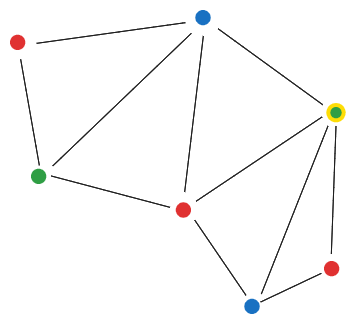
\includegraphics[width=0.6\textwidth,height=\textheight]{diagrams/complicated_gallery.png}
\caption{An example of a simple but difficult-to-optimise gallery
layout}
\end{figure}

Consider Fig. 3: Chvatal's proof shows that a maximum of three guards
(there are seven vertices, and the formula rounds up) are needed, and
Fisk's proof reduces that bound to at most two guards (these could be
placed at the two green vertices, or the two blue ones). However,
looking at the polygon, one can clearly see that only a single guard is
needed, placed at the highlighted green vertex. Human viewers can apply
a heuristic and observe that although the shape is concave, this vertex
can observe all of it. Every part of the polygon that the other green
vertex can observe, can also be observed by the highlighted vertex, plus
a bit more.

An algorithm to optimise this problem (minimising the number of guards)
would look at every combination of guard placements to see if the number
of guards can be reduced (a brute-force approach). Heuristics could be
applied, for example by counting around vertices and considering corner
angles relative to the origin vertex to see if they are occluded
(invisible from that point). A dynamic approach could also be used:
checking for each vertex, which other vertices are visible to it, and
iteratively eliminating those with poorest visibility to narrow the
search space (using Fisk's limit to restrict the search space as well).

Approximation methods sometimes use a grid to check the coverage of the
polygon from certain vertices in the shape, which could be resolved to
smaller granularities to more precisely map the space as needed,
although even this approach has been found to be NP-hard (Biedl et. al.,
2012)\footnote{Biedl, T.~\emph{et al.}~(2012) \emph{`The Art Gallery
  Theorem for Polyominoes.'}~\emph{Discrete \& Computational
  Geometry},~48, pp.~711--720. https://doi.org/10.1007/s00454-012-9429-1}.

One approach presented is to reduce the the overall polygon to a set of
convex polygons, each of which may be observed by a single guard (Ghosh,
1987)\footnote{Ghosh, S. K. (1987), \emph{`Approximation algorithms for
  art gallery problems'},~\emph{Proc. Canadian Information Processing
  Society Congress}, pp.~429--434.}. However, even this may not produce
optimal results, see Fig. 3 again.

It's important to note that there are several variations of the problem
which allow guards to be placed on edges, or even anywhere within the
polygon, and which allow/disallow holes in the polygon (which are
analogous to pillars in a gallery). Polygons may also be restricted to
being orthogonal (i.e.~having all squared edges); all of these
combinations of conditions affect the number of possible configurations
and methods for verifying solutions, though nearly all have been proven
NP-hard (Kröller et al, 2012)\footnote{Kröller, A.~\emph{et al.}~(2012)
  \emph{`Exact Solutions and Bounds for General Art Gallery
  Problems'},~\emph{ACM J. Exp. Algorithmics}. New York, NY, USA:
  Association for Computing Machinery, 17. doi:10.1145/2133803.2184449.},
(Schuchardt and Hecker, 1995)\footnote{Schuchardt, D., Hecker, H.D.
  (1995). \emph{`Two NP‐Hard Art‐Gallery Problems for
  Ortho‐Polygons.'}~\emph{Mathematical Logic Quarterly},~41(2),
  pp.~261-267. doi:10.1002/malq.19950410212.}.

One application of the art gallery problem is laser-scanning of
interiors, where the goal is to minimise the number of scans taken
(Kröller et al, 2012)\footnote{Kröller, A.~\emph{et al.}~(2012)
  \emph{`Exact Solutions and Bounds for General Art Gallery
  Problems'},~\emph{ACM J. Exp. Algorithmics}. New York, NY, USA:
  Association for Computing Machinery, 17. doi:10.1145/2133803.2184449.},
which means placing the `guards' anywhere inside the polygon. Another
example is generating navigation routes for autonomous robotics in
environments with many obstacles/holes (Lulu \& Elnagar,
2007)\footnote{Lulu, L., Elnagar, A. (2007) \emph{`An art gallery-based
  approach: Roadmap construction and path planning in global
  environments'}, \emph{International Journal of Robotics and
  Automation}, 22(4). doi:10.2316/journal.206.2007.4.206-3059.}.

\newpage

\subsection{Bibliography}\label{bibliography}

Chvátal, V. (2004) \emph{`A combinatorial theorem in plane geometry'},
\emph{Journal of Combinatorial Theory, Series B}. Available at:
https://www.sciencedirect.com/science/article/pii/0095895675900611
(Accessed: 29 October 2023).

Aigner, M., Ziegler, G.M. (2018). \emph{`How to guard a museum. In:
Proofs from THE BOOK'}. Springer, Berlin, Heidelberg.
https://doi.org/10.1007/978-3-662-57265-8\_40.

Ghosh, S. K. (1987), \emph{`Approximation algorithms for art gallery
problems'},~\emph{Proc. Canadian Information Processing Society
Congress}, pp.~429--434.

Flood, M. M. (1956), \emph{`The Traveling-Salesman Problem.',}
\emph{Operations Research}, 4(1), pp.~61--75. Available at:
http://www.jstor.org/stable/167517 (Accessed: 20 November 2023).

Bellman, R. (1962) \emph{`Dynamic programming treatment of the
travelling salesman problem'}, \emph{Journal of the ACM}, 9(1),
pp.~61--63. doi:10.1145/321105.321111.

Lee, D. and Lin, A. (1986) \emph{`Computational complexity of art
gallery problems'},~\emph{IEEE Transactions on Information Theory},
32(2), pp.~276--282. doi:10.1109/TIT.1986.1057165.

Hoare, C. A. R. (1962) \emph{`Quicksort'},~\emph{The Computer Journal},
5(1), pp.~10--16. doi:10.1093/comjnl/5.1.10.

Esau Taiwo, O. \emph{et al.} (2020) \emph{`Comparative study of two
divide and conquer sorting algorithms: Quicksort and Mergesort'},
\emph{Procedia Computer Science}, 171, pp.~2532--2540.
doi:10.1016/j.procs.2020.04.274.

Deshmukh, S.M., Bhavsar, A.K. (2020) \emph{`A Review on Different
Quicksort Algorithms'}, \emph{International Journal of Science,
Spirituality, Business and Technology}, 7(2), pp.~3--7.

Fouz, M. \emph{et al.} (2011) \emph{`On smoothed analysis
of~quicksort~and~Hoare's find'}, \emph{Algorithmica}, 62(3--4),
pp.~879--905. doi:10.1007/s00453-011-9490-9.

Abdulkarim, H.A., Alshammari, I.F., (2015) \emph{`Comparison of
algorithms for solving traveling salesman problem.'}~\emph{International
Journal of Engineering and Advanced Technology},~4(6), pp.~76-79.

Kizilateş, G., Nuriyeva, F. (2013) \emph{`On the nearest neighbor
algorithms for the traveling salesman problem'}, \emph{Advances in
Intelligent Systems and Computing}, pp.~111--118.
doi:10.1007/978-3-319-00951-3\_11.

Vince, A. (2002) \emph{`A framework for the greedy algorithm'},
\emph{Discrete Applied Mathematics}, 121(1--3), pp.~247--260.
doi:10.1016/s0166-218x(01)00362-6.

Poonthalir, G., Nadarajan, R. (2018) \emph{`A fuel efficient green
vehicle routing problem with varying speed constraint (F-GVRP)'},
\emph{Expert Systems with Applications}, 100, pp.~131--144.
doi:10.1016/j.eswa.2018.01.052.

Michael, T.S., Pinciu, V. (2016) \emph{`The orthogonal art gallery
theorem with Constrained Guards'}, \emph{Electronic Notes in Discrete
Mathematics}, 54, pp.~27--32. doi:10.1016/j.endm.2016.09.006.

Garey, M.R., Johnson, D.S., Preparata, F.P., Tarjan, R.E. (1978)
\emph{`Triangulating a simple polygon.'},~\emph{Information Processing
Letters},~7(4), pp.~175-179.

O'Rourke, J. (2012) \emph{Art Gallery Theorems and Algorithms},
\emph{Art Gallery theorems and algorithms}. Available at:
http://www.science.smith.edu/\textasciitilde jorourke/books/ArtGalleryTheorems/art.html
(Accessed: 23 November 2023).

Biedl, T.~\emph{et al.}~(2012) \emph{`The Art Gallery Theorem for
Polyominoes.'}~\emph{Discrete \& Computational Geometry},~48,
pp.~711--720. https://doi.org/10.1007/s00454-012-9429-1.

Kröller, A.~\emph{et al.}~(2012) \emph{`Exact Solutions and Bounds for
General Art Gallery Problems'},~\emph{ACM J. Exp. Algorithmics}. New
York, NY, USA: Association for Computing Machinery, 17.
doi:10.1145/2133803.2184449.

Schuchardt, D., Hecker, H.D. (1995). \emph{`Two NP‐Hard Art‐Gallery
Problems for Ortho‐Polygons.'}~\emph{Mathematical Logic
Quarterly},~41(2), pp.~261-267. doi:10.1002/malq.19950410212.

Lulu, L., Elnagar, A. (2007) \emph{`An art gallery-based approach:
Roadmap construction and path planning in global environments'},
\emph{International Journal of Robotics and Automation}, 22(4).
doi:10.2316/journal.206.2007.4.206-3059.

Rust, J. (2008) \emph{`Dynamic programming.'}~\emph{The new Palgrave
dictionary of economics},~1, p.~8.

Montero, A., Méndez-Díaz, I., Miranda-Bront, J.J. (2017) \emph{`An
integer programming approach for the time-dependent traveling salesman
problem with time windows'}, \emph{Computers \& Operations Research},
88, pp.~280--289. doi:10.1016/j.cor.2017.06.026.

Bensmail, J.~\emph{et al.}~(2019) \emph{`Backbone colouring and
algorithms for TDMA scheduling'},~\emph{Discrete Mathematics \&
Theoretical Computer Science}, 21(3). doi:10.23638/DMTCS-21-3-24.

\end{document}
